\chapter{Arithmétique dans $\mathbb{Z}$}

\begin{citationchapitre}
	« Dieu a créé les nombres entiers ; tout le reste est l'œuvre de l'homme. »
	
	--- Leopold Kronecker
\end{citationchapitre}

\begin{objectifs}
	\begin{itemize}[label=\textbullet]
		\item Maîtriser la divisibilité dans $\mathbb{Z}$.
		\item Utiliser le PGCD et le PPCM.
		\item Résoudre des congruences.
		\item Appliquer le théorème de Bézout.
		\item Appliquer le théorème de Gauss.
		\item Résoudre des équations diophantiennes simples.
	\end{itemize}
\end{objectifs}


\section{Divisibilité}
$\mathbb N$ est l'ensemble des entiers naturels
$\{0;1;2;\ldots\}$ ;

$\mathbb Z$ celui des entiers relatifs
$\{\ldots;-2;-1;0;1;2;\ldots\}$.
	\begin{definition}
		
		Soient $a$ et $b$ deux entiers relatifs avec $b\neq 0$.
		
		On dit que $b$ divise $a$, ou que $b$ est un diviseur de $a$,
		s'il existe un entier relatif $k$ tel que
		$$
		a=bk.
		$$
		
		On dit aussi que $a$ est un multiple de $b$.
		
	\end{definition}
	
	\begin{remarque}
		
		$0$ est un multiple de n'importe quel entier relatif $b$
		(car $0=b\times 0$).
		
		En revanche, $0$ n'est un diviseur d'aucun nombre.
		
	\end{remarque}
	
	\begin{exemple}
		
		$4$ divise $24$ car $24=4\times6$;
		$-4$ divise aussi $24$ car $24=(-4)\times(-6)$. 		
		Ainsi, $24$ est un multiple de $4$ et de $-4$.
		
	\end{exemple}
	
	\begin{propriete}
		
		Soient $a$ et $b$ deux entiers relatifs avec $b\neq0$.
		
		\begin{itemize}[label=\textbullet]
			\item Si $b\mid a$, alors tout multiple de $a$ est un multiple de $b$.
			\item Si $b\mid a$, alors tout diviseur de $b$ est un diviseur de $a$.
		\end{itemize}
		
	\end{propriete}
		
	\begin{propriete}
		
		Soient $a,b\in\mathbb Z$ avec $b\neq0$.
		
		$b\mid a\iff -b\mid a\iff b\mid(-a)\iff -b\mid(-a).$
		
	\end{propriete}
	
	$a$ et $-a$ ont les mêmes diviseurs dans $\mathbb Z$. Les diviseurs de $-a$ étant les opposés des diviseurs positifs de $a$, on restreindra souvent l'étude à la divisibilité dans $\mathbb N$.
	
	\consequence
	$a$ et $-a$ ont les mêmes diviseurs dans $\mathbb Z$. Les diviseurs de $-a$ étant les opposés des diviseurs positifs de $a$, on restreindra souvent l'étude à la divisibilité dans $\mathbb N$.
	
	\begin{propriete}
		
		\begin{enumerate}
			\item $a\mid b$ et $b\mid c \Rightarrow a\mid c$.
			
			\item $a\mid b$ et $a\mid c \Rightarrow a\mid(bu+cv)$ pour tous
			$u,v\in\mathbb Z$.
			
		\end{enumerate}
		
	\end{propriete}
	\begin{exemple}
		
		Si $a$ divise deux entiers consécutifs $n$ et $n+1$, alors
		
		$a\mid((n+1)-n)$.
		
		Ainsi, $a\mid1$ et donc $a=1$ ou $a=-1$.
		
	\end{exemple}
	
	\exerciceresolu
	\textbf{Caractériser la divisibilité}
	
	\begin{enumerate}
		\item Montrer que $14p^2-35q$ est divisible par $7$ quels que soient les entiers relatifs $p$ et $q$.
		
		\item Déterminer les entiers naturels $n$ tels que $4$ divise $n+13$.
	\end{enumerate}
	
	\solution
	
	\begin{enumerate}
		\item Il faut montrer qu'il existe un entier $k$ tel que
		$$
		14p^2-35q=7k.
		$$
		Or,
		$$
		14p^2-35q=7(2p^2-5q).
		$$
		Comme $2p^2-5q\in\mathbb Z$, on conclut que $14p^2-35q$ est divisible par $7$.
		
		\item Si $4$ divise $n+13$, alors il existe $k\in\mathbb N$ tel que
		$$
		n+13=4k.
		$$
		Ainsi,
		$$
		n=4k-13.
		$$
		Comme $n\ge0$, on doit avoir
		$$
		4k-13\ge0
		\quad\Longleftrightarrow\quad
		k\ge4.
		$$
		Les solutions sont donc les entiers de la forme
		$$
		n=4k-13,\qquad (k\ge4),
		$$
		c'est-à-dire
		$$
		\{3,7,11,\ldots\}.
		$$
		
	\end{enumerate}
	\exerciceresolu
	
	\textbf{Utiliser un raisonnement par l'absurde : }
	Montrer que, quel que soit l'entier relatif $n$, $2n+5$ n'est jamais divisible par $2$.
	
	\solution
	Supposons que $2n+5$ soit divisible par $2$.
	
	Il existe alors $k\in\mathbb Z$ tel que
	$$
	2n+5=2k.
	$$
	D'où
	$$
	5=2(k-n).
	$$
	Ainsi, $5$ serait divisible par $2$, ce qui est impossible.
	Donc $2$ ne divise jamais $2n+5$.
	
	\exerciceresolu
	\textbf{Déterminer et utiliser la liste des diviseurs d'un nombre :}
	
	Déterminer dans $\mathbb Z$ la liste des diviseurs de $7$ et en déduire les entiers relatifs $n$ tels que $4n+1$ divise $7$.
	
	\solution
	$$
	D(7)=\{-7,-1,1,7\}.
	$$
	
	Si $4n+1$ divise $7$, alors
	$$
	4n+1\in D(7).
	$$
	On résout successivement :
	
	$4n+1=7 \Longrightarrow n=\frac32$(pas de solution dans $\mathbb Z$),
	
	$4n+1=-7 \Longrightarrow n=-2,$
	$4n+1=1 \Longrightarrow n=0,$
	
	$4n+1=-1 \Longrightarrow n=-\frac12$	(pas de solution dans $\mathbb Z$).
	
	Les solutions sont donc	$n=-2 \quad\text{ou}\quad n=0.$\\

	
	\exerciceresolu
	\textbf{Utiliser une combinaison linéaire :}
	
	Déterminer les entiers relatifs $n$ tels que $2n+1$ divise $n+13$.
	
	\solution : On cherche une combinaison linéaire de $2n+1$ et de $n+13$ indépendante de $n$ :
	$$
	(2n+1)-2(n+13)=-25.
	$$
	Ainsi, si $2n+1$ divise $n+13$, alors $2n+1$ divise $25$.
	
	Or
	$$
	D(25)=\{-25,-5,-1,1,5,25\}.
	$$
	On résout :
	$2n+1=-25 \Longrightarrow n=-13,
	$ ou $2n+1=-5 \Longrightarrow n=-3,
	$ ou $2n+1=-1 \Longrightarrow n=-1$ ou $2n+1=1\Longrightarrow n=0,
	$ ou $2n+1=5 \Longrightarrow n=2,
	$ ou $2n+1=25 \Longrightarrow n=12.$\\
	Les solutions sont donc
	$$
	\boxed{\{-13,-3,-1,0,2,12\}}.
	$$
	
	
\section{Division euclidienne}

\begin{theoreme}
	Soient $a$ un entier relatif et $b$ un entier naturel non nul.
	
	Il existe un unique couple $(q,r)\in\mathbb Z\times\mathbb N$ tel que
	$$
	a=bq+r
	\qquad\text{avec}\qquad
	0\le r<b.
	$$
	Le nombre $q$ est le quotient et $r$ le reste de la division euclidienne de $a$ par $b$.
\end{theoreme}

\interpretationgraphique
On encadre $a$ par deux multiples consécutifs de $b$. \\
\begin{center}
	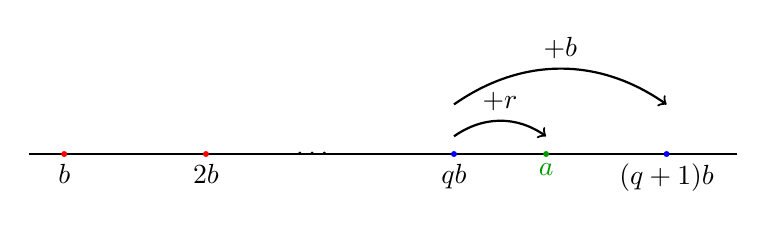
\begin{tikzpicture}[scale=0.9]
		
		% Axe
		\draw[thick] (0,0)--(10,0);
		
		% Points
		\fill[red] (0.5,0) circle (1.2pt);
		\fill[red] (2.5,0) circle (1.2pt);
		\fill[blue] (6,0) circle (1.2pt);
		\fill[green!60!black] (7.3,0) circle (1.2pt);
		\fill[blue] (9,0) circle (1.2pt);
		
		% Labels
		\node[below] at (0.5,0) {$b$};
		\node[below] at (2.5,0) {$2b$};
		\node[below] at (6,0) {$qb$};
		\node[below,green!60!black] at (7.3,0) {$a$};
		\node[below] at (9,0) {$(q+1)b$};
		
		\node at (4,0) {$\cdots$};
		
		% Arc r
		\draw[->,thick]
		(6,0.25) to[bend left=35] node[above] {$+r$} (7.3,0.25);
		
		% Arc b
		\draw[->,thick]
		(6,0.7) to[bend left=35] node[above] {$+b$} (9,0.7);
		
	\end{tikzpicture}
\end{center}


\begin{exemple}
	
	La division euclidienne de $114$ par $8$ est
	$$
	114=8\times14+2,
	$$
	avec $q=14$ et $r=2$ puisque $0\le2<8$.
\end{exemple}

\remarque
	\begin{itemize}[label=\textbullet]
		\item Dans la division euclidienne par $b$, il y a $b$ restes possibles : $0,1,2,\ldots b-1$.
		
		\item Il existe plusieurs écritures de la forme $a=bq+r$, mais une seule vérifie $0\le r<b$.
		Par exemple :
		$$
		56=17\times3+5=17\times2+22.
		$$
		Comme $22>17$, la seconde égalité n'est pas une division euclidienne.
		
	\end{itemize}
	
\begin{propriete}
	
	Soient $a\in\mathbb Z$ et $b\in\mathbb N^*$.
	
	$b$ divise $a$ si et seulement si le reste de la division euclidienne de $a$ par $b$ est nul.
\end{propriete}

\begin{exemple}
	$$
	-36=6\times(-6)+0
	$$
	est la division euclidienne de $-36$ par $6$.
	Ainsi, $6$ est un diviseur de $-36$.
\end{exemple}
\begin{propriete}
	
	Soit $b\ge2$ un entier naturel.
	
	Tout entier relatif s'écrit sous l'une des formes
	$$
	bq,\ bq+1,\ bq+2,\ \ldots,\ bq+(b-1)q
	$$ 	
	où $q\in\mathbb Z$.
\end{propriete}
\begin{exemple}
	Montrons que, pour tout entier relatif $n$, le nombre $n^2+1$ n'est jamais divisible par $3$.\\
	On utilise la propriété précédente pour raisonner par disjonction de cas.\\
	Tout entier s'écrit sous l'une des formes
	$3q$, $3q+1$ ou $3q+2$.
	
	\begin{itemize}[label=\textbullet]
		
		\item Si $n=3q$, $n^2+1=(3q)^2+1=9q^2+1 \neq 3k.$
		
		\item Si $n=3q+1$, $n^2+1=(3q+1)^2+1=9q^2+6q+2 \neq 3k.
		$		
		\item Si $n=3q+2, n^2+1=(3q+2)^2+1=9q^2+12q+5 \neq 3k.$
		
	\end{itemize}
	
	Dans les trois cas, $n^2+1$ n'est pas divisible par $3$.
	
\end{exemple}
	
\exerciceresolu
\textbf{Raisonner par disjonction des cas :}

Montrer que le produit de trois entiers naturels consécutifs est divisible par $3$.

\solution : Soit $n\in\mathbb N$. On veut montrer que
$(n-1)n(n+1)$ est divisible par $3$.

Tout entier s'écrit sous l'une des formes $3q$, $3q+1$ ou $3q+2$.

\begin{itemize}[label=\textbullet]
	
	\item Si $n=3q$, alors
	$$
	(n-1)n(n+1)=(3q-1)\times3q\times(3q+1)
	=3(3q-1)q(3q+1).
	$$
	\item Si $n=3q+1$, alors
	$$
	(n-1)n(n+1)=3q(3q+1)(3q+2)
	=3q(3q+1)(3q+2).
	$$
	\item Si $n=3q+2$, alors
	$$
	(n-1)n(n+1)=(3q+1)(3q+2)(3q+3)
	=3(3q+1)(3q+2)(q+1).
	$$
	
\end{itemize}

Dans les trois cas, $(n-1)n(n+1)$ est divisible par $3$.
	
\exerciceresolu
\textbf{Conjecturer une divisibilité :}

Conjecturer les valeurs de l'entier naturel $n$ pour lesquelles $n^2-1$ est divisible par $8$ et démontrer cette conjecture.

\solution : On calcule $n^2-1$ pour quelques valeurs de $n$ : on obtient : $-1,\;0,\;3,\;8,\;15,\;24,\;35,\;48,\ldots$

On conjecture que $n^2-1$ est divisible par $8$ lorsque $n$ est impair.

Si $n=2k$, alors
$$
n^2-1=4k^2-1,
$$
qui est impair, donc non divisible par $8$.

Si $n=2k+1$, alors
$$
n^2-1=(2k+1)^2-1=4k(k+1).
$$
Or $k$ et $k+1$ sont consécutifs, donc l'un des deux est pair :
$$
k(k+1)=2m.
$$
Ainsi,
$$
n^2-1=8m.
$$
Donc $n^2-1$ est divisible par $8$.
\[
\boxed{\;8\mid(n^2-1)\iff n\text{ est impair.}\;}
\]

\section{Congruences}
% ============================================================
%   SECTION : Congruences dans Z
%   Chapitre : Arithmétique dans Z  —  Mazava Maths
% ============================================================

\section{Congruences dans $\Z$}

\subsection{Définition et premières propriétés}

\begin{definition}
	Soient $a$ et $b$ deux entiers relatifs et $n$ un entier naturel non nul.
	
	On dit que $a$ est \textbf{congru à $b$ modulo $n$}, et on note
	$$
	a \equiv b \pmod{n} \quad \text{ou} \quad a \equiv b\ [n],
	$$
	lorsque $a - b$ est un multiple de $n$, c'est-à-dire lorsqu'il existe $k \in \Z$ tel que $a - b = kn$.
\end{definition}

\begin{exemple}
	\begin{itemize}[label=\textbullet]
		\item $15 - 7 = 8 = 2 \times 4$, donc $15 \equiv 7\ [2]$ et $15 \equiv 7\ [4]$.
		\item $-5 - (-1) = -4 = -1 \times 4$, donc $-5 \equiv -1\ [4]$.
	\end{itemize}
\end{exemple}

\remarque
$a \equiv b\ [n] \iff b \equiv a\ [n]$. On dit aussi que $a$ et $b$ sont \textbf{congrus modulo $n$}.

\begin{propriete}
	Soient $a$ et $b$ deux entiers relatifs et $n$ un entier naturel non nul.
	
	$a \equiv b\ [n]$ si et seulement si $a$ et $b$ ont le même reste dans la division euclidienne par $n$.
\end{propriete}

\begin{exemple}
	$11 = 4 \times 2 + 3$ et $7 = 4 \times 1 + 3$, avec $0 \leqslant 3 < 4$.
	
	Donc $11$ et $7$ ont tous deux le reste $3$ dans la division par $4$, et donc $11 \equiv 7\ [4]$.
\end{exemple}

\begin{propriete}
	Soient $a$, $b$, $c$ des entiers relatifs et $n$ un entier naturel non nul.
	\begin{enumerate}
		\item $a \equiv 0\ [n]$ si et seulement si $n \mid a$.
		\item $a \equiv a\ [n]$ \quad (réflexivité).
		\item $r$ est le reste de la division euclidienne de $a$ par $n$ si et seulement si
		$a \equiv r\ [n]$ et $0 \leqslant r < n$.
		\item Si $a \equiv b\ [n]$ et $b \equiv c\ [n]$, alors $a \equiv c\ [n]$ \quad (transitivité).
	\end{enumerate}
\end{propriete}

\begin{exemple}
	\begin{itemize}[label=\textbullet]
		\item $12 \equiv 0\ [2]$. On a aussi $12 \equiv 0\ [3]$ et $12 \equiv 0\ [6]$.
		\item $13 \equiv -5\ [2]$ et $-5 \equiv -1\ [2]$, donc $13 \equiv -1\ [2]$ par transitivité.
	\end{itemize}
\end{exemple}

%--------------------------------------------------------------
\subsection{Calculs avec les congruences}
%--------------------------------------------------------------

\begin{propriete}[Compatibilité avec les opérations]
	Soient $a$, $b$, $c$, $d$ des entiers relatifs et $n$ un entier naturel non nul.
	
	\begin{enumerate}
		\item Si $a \equiv b\ [n]$, alors $a + c \equiv b + c\ [n]$.
		
		\item Si $a \equiv b\ [n]$ et $c \equiv d\ [n]$, alors $a + c \equiv b + d\ [n]$.
		
		On dit que \textbf{l'addition est compatible avec les congruences}.
		
		\item Si $a \equiv b\ [n]$, alors $ac \equiv bc\ [n]$.
		
		\item Si $a \equiv b\ [n]$ et $c \equiv d\ [n]$, alors $ac \equiv bd\ [n]$.
		
		On dit que \textbf{la multiplication est compatible avec les congruences}.
		
		\item Si $a \equiv b\ [n]$, alors pour tout entier naturel non nul $p$,
		$$
		a^p \equiv b^p\ [n].
		$$
	\end{enumerate}
\end{propriete}

\begin{exemple}
	\begin{itemize}[label=\textbullet]
		\item $x + 2 \equiv 3\ [4]$ et $-2 \equiv -2\ [4]$, donc $x + 2 - 2 \equiv 3 - 2\ [4]$,
		d'où $x \equiv 1\ [4]$.
		\item $10 \equiv 1\ [9]$, donc $10^p \equiv 1^p \equiv 1\ [9]$ pour tout entier naturel non nul $p$.
	\end{itemize}
\end{exemple}

\begin{attention}
	La division n'est pas compatible avec les congruences.
	
	Par exemple, $5 \times 4 \equiv 5 \times 6\ [10]$ (car $20 \equiv 30\ [10]$), mais $4 \not\equiv 6\ [10]$.
\end{attention}

%--------------------------------------------------------------
\subsection{Méthodes et exercices résolus}
%--------------------------------------------------------------

\exerciceresolu
\textbf{Résoudre des équations avec des congruences}

Résoudre les équations suivantes dans $\Z$ :
\begin{enumerate}
	\item $x + 3 \equiv 2\ [7]$
	\item $3x \equiv 2\ [5]$
	\item $x^2 \equiv 0\ [4]$
\end{enumerate}

\solution

\begin{enumerate}
	\item Par compatibilité avec l'addition :
	$$
	x + 3 \equiv 2\ [7]
	\iff x + 3 - 3 \equiv 2 - 3\ [7]
	\iff x \equiv -1\ [7].
	$$
	Les solutions sont donc les entiers de la forme $7k - 1$ avec $k \in \Z$.
	
	\item On utilise un tableau de congruences modulo $5$ :
	\[
	\begin{array}{|c|c|c|c|c|c|}
		\hline
		x \equiv \ldots\ [5] & 0 & 1 & 2 & 3 & 4 \\
		\hline
		3x \equiv \ldots\ [5] & 0 & 3 & 1 & 4 & 2 \\
		\hline
	\end{array}
	\]
	Le seul cas qui convient est $x \equiv 4\ [5]$.
	
	Les solutions sont donc les entiers de la forme $5k + 4$ avec $k \in \Z$.
	
	\item On raisonne par disjonction des cas modulo $4$ :
	\[
	\begin{array}{|c|c|c|c|c|}
		\hline
		x \equiv \ldots\ [4] & 0 & 1 & 2 & 3 \\
		\hline
		x^2 \equiv \ldots\ [4] & 0 & 1 & 0 & 1 \\
		\hline
	\end{array}
	\]
	Deux cas conviennent : $x \equiv 0\ [4]$ et $x \equiv 2\ [4]$.
	
	Les solutions sont donc les entiers de la forme $4k$ ou $4k + 2$ avec $k \in \Z$.
\end{enumerate}


\exerciceresolu
\textbf{Montrer une divisibilité à l'aide des congruences}

\begin{enumerate}
	\item Montrer que pour tout entier naturel $n$ non nul, $2^{3n} - 1$ est un multiple de $7$.
	\item Déterminer les valeurs de l'entier naturel $n$ pour lesquelles $n^2 - 3n + 6$ est divisible par $4$.
\end{enumerate}

\solution

\begin{enumerate}
	\item On a $2^3 = 8$ et $8 = 7 + 1$, donc $8 \equiv 1\ [7]$, c'est-à-dire $2^3 \equiv 1\ [7]$.
	
	Par compatibilité avec les puissances :
	$$
	2^{3n} = \left(2^3\right)^n \equiv 1^n \equiv 1\ [7].
	$$
	Donc $2^{3n} - 1 \equiv 0\ [7]$, ce qui signifie que $2^{3n} - 1$ est bien un multiple de $7$.
	
	\item On utilise un tableau de congruences modulo $4$ :
	\[
	\begin{array}{|c|c|c|c|c|}
		\hline
		n \equiv \ldots\ [4] & 0 & 1 & 2 & 3 \\
		\hline
		n^2 \equiv \ldots\ [4] & 0 & 1 & 0 & 1 \\
		\hline
		3n \equiv \ldots\ [4] & 0 & 3 & 2 & 1 \\
		\hline
		n^2 - 3n + 6 \equiv \ldots\ [4] & 2 & 0 & 0 & 2 \\
		\hline
	\end{array}
	\]
	Les entiers $n$ qui conviennent sont donc ceux de la forme $4k + 1$ ou $4k + 2$ avec $k \in \N$.
\end{enumerate}

\exerciceresolu
\textbf{Déterminer le reste d'une division euclidienne}

Déterminer le reste de la division euclidienne de $11^{2020}$ par $3$.

\solution

On a $11 \equiv 2\ [3]$, puis $11^2 = 121 \equiv 4 \equiv 1\ [3]$.

Donc pour tout entier $q > 0$ :
$$
11^{2q} = \left(11^2\right)^q \equiv 1^q \equiv 1\ [3].
$$
Or $2020 = 2 \times 1010$ est de la forme $2q$, donc $11^{2020} \equiv 1\ [3]$.

Comme $0 \leqslant 1 < 3$, le reste de la division euclidienne de $11^{2020}$ par $3$ est $\boxed{1}$.

\begin{astucebac}
	Pour calculer le reste de $a^n$ modulo $p$, on cherche d'abord une petite puissance de $a$
	congrue à $1$ (ou à une valeur simple) modulo $p$, puis on écrit $n$ sous une forme adaptée.
	Cette technique s'appelle la \textbf{méthode des puissances successives}.
\end{astucebac}

% ============================================================
%  SECTIONS : PGCD — Bézout — Gauss — Équations diophantiennes
%  Chapitre : Arithmétique dans Z  —  Mazava Maths
% ============================================================


% ------------------------------------------------------------
\section{PGCD et algorithme d'Euclide}
% ------------------------------------------------------------

\begin{definition}
	Soient $a$ et $b$ deux entiers naturels non tous les deux nuls.
	
	L'ensemble $D(a\,;b) = D(a) \cap D(b)$ des diviseurs communs de $a$ et $b$ admet
	un plus grand élément, noté $\mathrm{PGCD}(a\,;b)$, appelé \textbf{plus grand commun diviseur}
	de $a$ et de $b$.
	
	Par convention, si $a \in \N^*$, alors $\mathrm{PGCD}(a\,;0) = a$.
\end{definition}

\remarque
Si $a$ et $b$ sont deux entiers \emph{relatifs}, on pose
$\mathrm{PGCD}(a\,;b) = \mathrm{PGCD}(|a|\,;|b|)$.

\begin{exemple}
	$D(9\,;15) = \{-3\,;-1\,;1\,;3\}$, donc $\mathrm{PGCD}(9\,;15) = 3$.
\end{exemple}

\begin{propriete}[Algorithme d'Euclide]
	Soient $a$ et $b$ deux entiers naturels non nuls et $r$ le reste de la division euclidienne
	de $a$ par $b$.
	$$
	D(a\,;b) = D(b\,;r), \quad \text{donc} \quad \mathrm{PGCD}(a\,;b) = \mathrm{PGCD}(b\,;r).
	$$
	On effectue des divisions euclidiennes successives jusqu'à obtenir un reste nul :
	le \textbf{PGCD} est alors le \textbf{dernier reste non nul}.
\end{propriete}

\exerciceresolu
\textbf{Déterminer un PGCD par l'algorithme d'Euclide}

Déterminer $\mathrm{PGCD}(1\,551\,;\,132)$.

\solution

On effectue les divisions euclidiennes successives :
$$
1\,551 = 11 \times 132 + 99
$$
$$
132 = 1 \times 99 + 33
$$
$$
99 = 3 \times 33 + 0
$$
Le dernier reste non nul est $33$, donc $\mathrm{PGCD}(1\,551\,;\,132) = 33$.

\begin{propriete}[Homogénéité du PGCD]
	Soient $a$ et $b$ deux entiers relatifs non nuls et $k$ un entier naturel non nul.
	$$
	\mathrm{PGCD}(ka\,;kb) = k\,\mathrm{PGCD}(a\,;b).
	$$
\end{propriete}

\begin{exemple}
	$\mathrm{PGCD}(60\,;90) = \mathrm{PGCD}(30 \times 2\,;\,30 \times 3)
	= 30 \times \mathrm{PGCD}(2\,;3) = 30 \times 1 = 30$.
\end{exemple}


% ------------------------------------------------------------
\section{Nombres premiers entre eux et théorème de Bézout}
% ------------------------------------------------------------

\begin{definition}
	Soient $a$ et $b$ deux entiers relatifs non nuls.
	
	On dit que $a$ et $b$ sont \textbf{premiers entre eux} lorsque $\mathrm{PGCD}(a\,;b) = 1$.
\end{definition}

\remarque
Les seuls diviseurs communs de deux entiers premiers entre eux sont $-1$ et $1$.

\begin{definition}
	Soient $a$ un entier relatif et $b$ un entier naturel non nul.
	
	La fraction $\dfrac{a}{b}$ est \textbf{irréductible} si $a$ et $b$ sont premiers entre eux.
\end{definition}

\begin{propriete}
	Soient $a$ et $b$ deux entiers relatifs non nuls et $d = \mathrm{PGCD}(a\,;b)$.
	
	Il existe deux entiers $a'$ et $b'$ tels que $a = da'$, $b = db'$ et $\mathrm{PGCD}(a'\,;b') = 1$.
\end{propriete}

\begin{theoreme}[Théorème de Bézout]
	Soient $a$ et $b$ deux entiers relatifs non nuls.
	
	$a$ et $b$ sont premiers entre eux si et seulement s'il existe deux entiers relatifs $u$ et $v$ tels que
	$$
	au + bv = 1.
	$$
\end{theoreme}

\begin{exemple}
	$1 \times 128 + (-1) \times 127 = 1$, donc $127$ et $128$ sont premiers entre eux.
\end{exemple}

\remarque
Le théorème de Bézout assure l'existence de $u$ et $v$, mais ne les fournit pas.
On peut les calculer en « remontant » les étapes de l'algorithme d'Euclide.

\begin{theoreme}[Bézout généralisé]
	Soient $a$ et $b$ deux entiers relatifs non nuls.
	
	$\mathrm{PGCD}(a\,;b) = d$ si et seulement si $d$ divise $a$ et $b$, et s'il existe deux entiers
	relatifs $u$ et $v$ tels que $au + bv = d$.
\end{theoreme}

\remarque
La condition «$d$ divise $a$ et $b$» est indispensable.
Par exemple $5 = 3 \times 1 + 2 \times 1$, mais $5$ n'est pas le PGCD de $3$ et $2$.


% ------------------------------------------------------------
\section{Théorème de Gauss}
% ------------------------------------------------------------

\begin{theoreme}[Théorème de Gauss]
	Soient $a$, $b$ et $c$ trois entiers relatifs non nuls.
	
	Si $a$ divise $bc$ et si $a$ et $b$ sont premiers entre eux, alors $a$ divise $c$.
\end{theoreme}

\remarque
La condition «$a$ et $b$ premiers entre eux» est indispensable.
Par exemple, $4$ divise $12 = 2 \times 6$, mais $4$ ne divise ni $2$ ni $6$.

\begin{corollaire}
	Soient $a$, $b$ et $c$ trois entiers relatifs non nuls.
	
	Si $a$ divise $c$, si $b$ divise $c$, et si $a$ et $b$ sont premiers entre eux,
	alors $ab$ divise $c$.
\end{corollaire}

\begin{exemple}
	Soit $n$ un entier naturel et $N = n(n+1)(n+2)$.
	\begin{itemize}[label=\textbullet]
		\item $n$ et $n+1$ sont consécutifs, donc $2 \mid N$.
		\item $n$, $n+1$ et $n+2$ sont trois consécutifs, donc $3 \mid N$.
		\item Comme $\mathrm{PGCD}(2\,;3) = 1$, le corollaire donne $6 \mid N$.
	\end{itemize}
\end{exemple}


% ------------------------------------------------------------
\section{Équations diophantiennes}
% ------------------------------------------------------------

\begin{definition}
	Une \textbf{équation diophantienne} est une équation de la forme
	$$
	ax + by = c,
	$$
	où $a$, $b$, $c$ sont des entiers relatifs donnés et les inconnues $x$ et $y$ sont cherchées
	dans $\Z$.
\end{definition}

\begin{propriete}[Condition d'existence des solutions]
	Soient $a$, $b$ et $c$ trois entiers relatifs non nuls.
	
	L'équation $ax + by = c$ admet des solutions dans $\Z^2$ si et seulement si
	$\mathrm{PGCD}(a\,;b)$ divise $c$.
\end{propriete}

\begin{exemple}
	Comme $\mathrm{PGCD}(2\,;3) = 1$ divise tout entier, l'équation $2x + 3y = 1$ admet toujours
	des solutions.
\end{exemple}

\begin{methode}[Résoudre une équation diophantienne $ax + by = c$]
	\begin{enumerate}
		\item Vérifier que $\mathrm{PGCD}(a\,;b)$ divise $c$ (sinon, pas de solution).
		\item Trouver une \textbf{solution particulière} $(x_0\,;y_0)$ par tâtonnement ou en
		remontant l'algorithme d'Euclide.
		\item En déduire \textbf{toutes les solutions} : si $(x_0\,;y_0)$ est une solution particulière,
		alors l'ensemble des solutions est
		$$
		S = \left\{\left(x_0 + \frac{b}{d}\,k\ ;\ y_0 - \frac{a}{d}\,k\right),\ k \in \Z\right\},
		\quad \text{où } d = \mathrm{PGCD}(a\,;b).
		$$
	\end{enumerate}
\end{methode}

\exerciceresolu
\textbf{Résoudre une équation diophantienne}

Résoudre dans $\Z^2$ l'équation $(E) : 2x + 5y = 4$.

\solution

\textbf{Étape 1 — Existence.}
$\mathrm{PGCD}(2\,;5) = 1$ divise $4$, donc $(E)$ admet des solutions.

\textbf{Étape 2 — Solution particulière.}
On cherche $u$ et $v$ tels que $2u + 5v = 1$ :
$$
2 \times (-2) + 5 \times 1 = 1.
$$
En multipliant par $4$ : $2 \times (-8) + 5 \times 4 = 4$.

Donc $(x_0\,;y_0) = (-8\,;4)$ est une solution particulière de $(E)$.

\textbf{Étape 3 — Solutions générales.}
$(E)$ s'écrit $2(x - x_0) = 5(y_0 - y)$, soit $2(x+8) = 5(4-y)$.

Comme $\mathrm{PGCD}(2\,;5) = 1$, le théorème de Gauss donne $2 \mid (4-y)$,
donc $4 - y = 2k$ et $y = 4 - 2k$ pour un certain $k \in \Z$.

En remplaçant : $x + 8 = 5k$, soit $x = -8 + 5k$.

L'ensemble des solutions est :
$$
\boxed{S = \{(-8+5k\ ;\ 4-2k),\ k \in \Z\}.}
$$

\exerciceresolu
\textbf{Déterminer si une équation diophantienne admet des solutions}

Parmi les équations suivantes, lesquelles admettent des solutions dans $\Z^2$ ?
$$
(E_1) : 13x + 14y = 3 \qquad (E_2) : 39x - 42y = 2
$$

\solution

Pour $(E_1)$ : $14 \times 1 + 13 \times (-1) = 1$, donc $\mathrm{PGCD}(13\,;14) = 1$.
Comme $1$ divise $3$, l'équation $(E_1)$ \textbf{admet des solutions}.

Pour $(E_2)$ : $\mathrm{PGCD}(39\,;42) = \mathrm{PGCD}(39\,;42)$.
Or $42 = 1 \times 39 + 3$ et $39 = 13 \times 3 + 0$, donc $\mathrm{PGCD}(39\,;42) = 3$.
Comme $3$ ne divise pas $2$, l'équation $(E_2)$ \textbf{n'admet pas de solution}.


\section{Exercices}

